% ==========================================
% LatexRefinement Step Output: step4-04-28-25-tuesday-all-offset-final.tex
% Model: gemini-3.6-flash
% Temperature: 0.33
% TopP: 0.95
% TopK: 40
% MaxOutputTokens: 65535
% ThinkingBudget: 32765
% ThinkingLevel: HIGH
% Prompt Tokens: 59'616
% Candidates Tokens: 22'283 (inkl. Thinking Tokens)
% Cached Tokens: 0
% Processed on: 2026-07-22 20:17:49
% ==========================================

% Primary Language: German
% End of the video: 01:25:38

\lecturechapter[10]{Dienstag}{28. Apr}{28. April 2026}{Einführung in die Graphentheorie}

\begin{nice-box}[Vorlesungsüberblick \& Kontext]
In dieser Vorlesung schließt der Dozent das Kapitel über das Auswahlaxiom und die Kardinalzahlen ab und leitet in die \newterm{Graphentheorie} ein.

\textbf{Zentrale Themen der Vorlesung:}
\begin{itemize}
    \item \textbf{Historischer Hintergrund:} Das Königsberger Brückenproblem und Leonhard Eulers Paritätsargument.
    \item \textbf{Formalisierung von Graphen:} Knoten, Kanten, gerichtete und ungerichtete Graphen, Schlingen, Mehrfachkanten und schlichte Graphen.
    \item \textbf{Die Adjazenzmatrix:} Formalisierung, algebraische Eigenschaften (Spur, Symmetrie) und Anwendung bei Multigraphen.
    \item \textbf{Gradbegriffe \& Graphenklassen:} Halbgrade in Digraphen, Knotengrad im ungerichteten Fall, reguläre und vollständige Graphen ($K_n$) sowie induzierte Teilgraphen.
    \item \textbf{Wege, Züge \& Matrixpotenzen:} Pfeil- und Kantenzüge, Bahnen, Wege, Wirbel, Kreise und Pfeilfolgen sowie der Beweis von Proposition~\ref{prop:adjazenzmatrix-potenz-pfeilfolgen} ($A^k$ als Pfadzähler).
\end{itemize}
\end{nice-box}

\section{Organisatorisches und Überblick}

\begin{spoken-clean}[00:00:00 - 00:01:08]
Hallo zusammen und herzlich willkommen zur nächsten Woche von Grundstrukturen.

Wie ich das letzte Mal gesagt habe, schließen wir das Kapitel über das Auswahlaxiom und Kardinalzahlen jetzt ab. Im Skript sehen Sie, da gibt es noch zwei Kapitel über Nichtstandard-Analysis, die werden wir überspringen. Die sind nicht so standard. Aber wenn Sie Lust haben, da reinzuschauen: Es ist ein witziges Thema.

Es geht darum, Nichtstandardmodelle von den reellen Zahlen zu konstruieren; und dann kann man auf diesen Nichtstandardmodellen dennoch Analysis machen und diese Nichtstandardmodelle auch wieder verwenden, um Aussagen über die Standard-Analysis zu machen. Es ist ein witziges Thema, ja.
\end{spoken-clean}

\begin{student-interaction}[Studentenfrage]
Wenn wir das überspringen, ist das dann immer noch examensrelevant?
\end{student-interaction}

\begin{spoken-clean}[00:01:08 - 00:03:08]
Nein, ist nicht examensrelevant. Das Skript ist etwas länger als eine zweistündige Vorlesung, deswegen darf da jeder ein bisschen seine Auswahl treffen. Und vielleicht werden wir noch ein paar Sachen machen, die nicht im Skript sind; die werde ich Ihnen dann aber dazugeben.

Schauen Sie sich das an, wenn Sie sich für diese Sachen interessieren. Das ist lustig; Sie können auch weiterlesen, zum Beispiel im Buch von Lorenz Halbeisen und Regula Krapf.

Aber ja, wir machen jetzt direkt weiter im Kapitel über die Graphentheorie. Damit lassen wir jetzt vorerst einmal diese Logikgeschichten zurück --- obwohl, die lässt man natürlich nie zurück, weil natürlich die ganze Mathematik auf der Logik und auf Zermelo-Fraenkel aufbaut. Im Hintergrund verwenden wir diese ganzen Sachen natürlich immer noch: Man kann immer noch Signaturen anschauen und dann das Ganze entsprechend formulieren und so weiter. Und man kann auch alle Beweise, die wir führen, formalisieren und auf Zermelo-Fraenkel zurückführen. Das ist etwas, was Leute machen, zum Beispiel mit der Sprache Lean.

Um natürlich einigermaßen voranzukommen, werden wir die Sachen jetzt in --- wie soll ich sagen --- alltäglicher mathematischer Sprache diskutieren. Es geht also darum, dass Sie ein paar Grundbegriffe lernen: jetzt eben zuerst ein bisschen sehr elementare Graphentheorie, danach noch etwas sehr elementare Zahlentheorie, wahrscheinlich noch etwas über endliche Körper und, wenn wir Zeit haben, noch ein bisschen elementare Gruppentheorie. Einfach damit Sie da gewisse Sachen lernen, für die Sie in anderen Vorlesungen keine Zeit haben, und auch damit Sie ein bisschen einen Blick dafür bekommen, was es so gibt in der Mathematik. Und auch hier ist überall wieder wichtig, dass Sie die Übungen lösen; denn es geht darum, dass Sie lernen, saubere mathematische Argumente zu führen, was Sie nachher können sollten.
\end{spoken-clean}

\section{Einführung in die Graphentheorie}

\subsection{Historischer Hintergrund: Das Königsberger Brückenproblem}

\begin{spoken-clean}[00:03:08 - 00:05:40]
Gut, jetzt aber zur Graphentheorie. Ein bisschen Geschichte: Da gehen wir jetzt etwas weiter zurück, als wir das bis jetzt hatten bei den Leuten, denen wir begegnet sind.

Da gehen wir zurück zu Leonhard Euler, dem Sie bestimmt auch schon begegnet sind. Gewissermaßen auch ein Schweizer Mathematiker eigentlich --- also $1707$ in Basel geboren, noch sehr früh in der Mathematik. Damals gab es natürlich noch keine ETH, aber es gab natürlich schon seit Langem die Universität Basel, und das ist auch dort, wo er studiert hat. Damals waren die Bernoullis an der Uni Basel; das ist eine ganze Familiengeneration, die hatten immer wieder Lehrstühle, also über mehrere Generationen denselben Lehrstuhl, und die waren sehr einflussreich in der Entwicklung der Mathematik und der Physik.

Jeweils am Samstagnachmittag ging Euler, glaube ich, zu --- was war es, Johann Bernoulli? ---, und der hat ihm dann ein paar Sachen erklärt oder so. Ich glaube, Johann Bernoulli hatte nicht viel Zeit und hat ihm viele Sachen zu lesen gegeben, aber Euler hat einmal geschrieben, dass es wunderbar war: Er hat ein paar wenige Fragen gestellt, und die Art und Weise, wie Bernoulli ihm diese Sachen beantwortet hat, hat ihm direkt viele andere Fragen sofort geklärt.

Ja, er hat sich, glaube ich, als er noch sehr jung war, für eine Physik-Professur in Basel beworben, die er aber nicht bekommen hat. Dann ist er weg und leider nie mehr in die Schweiz zurückgekehrt --- akademisch. Er hat dann eine Professur in Sankt Petersburg bekommen --- damals war, glaube ich, noch ein anderer Bernoulli dort ---, war eine Zeit lang in Berlin und dann wieder in Sankt Petersburg.

Ich glaube, man kann fast nicht unterschätzen, wie wichtig Euler für viele moderne Begriffe in der Mathematik war; er hat viele Gebiete eigentlich fast neu erfunden. Und eines davon ist eben, dass er die Graphentheorie erfunden hat. Das begann mit dem folgenden Problem... Gewissermaßen kann man auch fast sagen, dass das die Erfindung der Topologie war.
\end{spoken-clean}

\begin{meta-note}[Projizierter Inhalt: Leonhard Euler]
Der Dozent projiziert ein Porträt von Leonhard Euler ($1707$--$1783$) und erläutert dessen historischen und mathematischen Hintergrund.
\end{meta-note}

\begin{spoken-clean}[00:05:40 - 00:08:07]
Das war das Königsberger Brückenproblem. Das war Königsberg im damaligen Preußen --- gehört im weitesten Sinne zu Deutschland, heutzutage heißt die Stadt Kaliningrad. Okay, das sieht so aus, wie es aussieht: Es gibt so eine Insel und zwei Flüsse, die da zusammenkommen. Die Stadt hat diese vier Teile, und da gab es diese Brücken --- wie viele Brücken? Sieben Brücken in der Stadt.

Die Leute sind dort gerne spazieren gegangen, und in der Stadt kursierte so diese Knobelaufgabe oder diese Frage: Gibt es einen Spaziergang, sodass man in dieser Stadt --- also am Sonntagnachmittag --- so spazieren gehen kann, dass man zwar über alle Brücken läuft, aber über jede Brücke nur einmal? Genau einmal. Und die Frage ist auch: Wenn ja, kann man das so machen, dass man am selben Ort wieder aufhört, wo man anfängt?

Bei sieben Brücken kann man sich gut vorstellen: Wenn da viele Leute in der Stadt darüber nachdenken und es eine solche Möglichkeit gäbe, dann wäre wahrscheinlich jemand darauf gekommen. Aber wie Sie vielleicht auch schon gehört haben: Für das Problem gibt es keine Lösung. Die Frage ist natürlich: weshalb?

Einer dieser Herren hat das, glaube ich, in einem Brief an Euler gefragt, und Euler hat zuerst geantwortet: \qt{Ja, spannende Frage, aber...} Er sagt so direkt, das habe gar nichts mit Mathematik zu tun; das könne eigentlich jeder... Ist eigentlich kein mathematisches Problem: Jeder, der mit gesundem Verstand denken kann, kann das lösen, da braucht man gar keine Mathematiker. Aber er hat dann trotzdem weitergedacht und das Problem gelöst.
\end{spoken-clean}

\begin{meta-note}[Projizierter Inhalt: Das Königsberger Brückenproblem]
Der Dozent zeigt einen historischen Stadtplan von Königsberg mit den sieben hervorgehobenen Brücken über die Pregel.
\end{meta-note}

\begin{spoken-clean}[00:08:07 - 00:09:33]
Aber der wesentliche Teil hier ist einfach diese Abstraktion, die Euler dann eben gemacht hat. Er hat gesagt: Okay, nehmen wir diese vier zusammenhängenden Landteile --- also diese eine Insel, dann den oberen Teil, da noch einen Teil, da noch einen Teil ---, wir schauen uns die jetzt einfach ganz abstrakt an, und die sind verbunden mit Brücken. Da gibt es eine Brücke, da gibt es eine Brücke, da gibt es eine Brücke, und da gibt es je zwei Brücken.

Wenn man das so anschaut... da spielt es gar keine Rolle... Das Wichtige ist einfach: Wie sind diese vier Knoten miteinander verbunden? Aber wie lange diese Wege sind oder wie das genau aussieht, spielt keine Rolle. Wir können darauf abstrahieren. Und dann --- Sie kennen das Argument: Wenn es einen Weg gäbe, sodass man wieder an denselben Ort zurückkommt, dann kommt man in jeden dieser Knoten: Wenn man reinkommt, geht man auch wieder raus. Das heißt, das kommt immer in Paaren. An jedem dieser Knoten muss also die Anzahl der Kanten, die von diesem Knoten ausgehen, gerade sein.

Aber hier haben wir $3$, hier haben wir $5$, hier haben wir $3$, hier haben wir $3$. Die sind alle nicht einmal gerade! Es kann also kein geschlossener Pfad existieren. Wenn einer existieren würde, der vielleicht einen anderen Anfangs- als Endpunkt hätte, wäre es wieder überall gerade außer am Anfangs- und Endpunkt. Aber das ist überall ungerade; das heißt, es gibt auch keinen Weg, bei dem man irgendwo anfängt. Okay, das war die Lösung des Königsberger Brückenproblems.
\end{spoken-clean}

\begin{math-stroke}[Das Königsberger Brückenproblem als Graph]
\begin{center}
\begin{tikzpicture}[scale=1.2, >=stealth, node distance=2.5cm, main node/.style={circle, draw, fill=MidnightBlue!10, font=\sffamily\bfseries}]
  \node[main node] (A) at (0, 2) {$A$};
  \node[main node] (B) at (0, 0) {$B$};
  \node[main node] (C) at (0, -2) {$C$};
  \node[main node] (D) at (3, 0) {$D$};

  % Edges between A and B (2 bridges)
  \draw[thick, BrickRed] (A) to[bend left=30] node[left] {\footnotesize $e_1$} (B);
  \draw[thick, BrickRed] (A) to[bend right=30] node[right] {\footnotesize $e_2$} (B);

  % Edges between B and C (2 bridges)
  \draw[thick, BrickRed] (B) to[bend left=30] node[left] {\footnotesize $e_3$} (C);
  \draw[thick, BrickRed] (B) to[bend right=30] node[right] {\footnotesize $e_4$} (C);

  % Single edges to D
  \draw[thick, BrickRed] (A) to[bend left=20] node[above right] {\footnotesize $e_5$} (D);
  \draw[thick, BrickRed] (B) -- node[above] {\footnotesize $e_6$} (D);
  \draw[thick, BrickRed] (C) to[bend right=20] node[below right] {\footnotesize $e_7$} (D);

  % Node Degrees
  \node[above=0.2cm of A, ForestGreen] {\footnotesize $\operatorname{deg}(A) = 3$};
  \node[left=0.5cm of B, ForestGreen] {\footnotesize $\operatorname{deg}(B) = 5$};
  \node[below=0.2cm of C, ForestGreen] {\footnotesize $\operatorname{deg}(C) = 3$};
  \node[right=0.2cm of D, ForestGreen] {\footnotesize $\operatorname{deg}(D) = 3$};
\end{tikzpicture}
\end{center}

\begin{explanation-of-steps}[Eulersches Paritätsargument für den Königsberger Multigraphen]
Die vier Landmassen werden als Knoten $V = \{A, B, C, D\}$ modelliert, die sieben Brücken als Kanten.
\begin{itemize}
    \item \textbf{Geschlossener Eulerweg:} Bei jedem Betreten eines Knotens muss dieser über eine andere Kante wieder verlassen werden. Jeder Durchgang verbraucht somit $2$ Kanten. Ein geschlossener Eulerweg setzt voraus, dass der Grad jedes Knotens $\operatorname{deg}(v)$ gerade ist.
    \item \textbf{Offener Eulerweg:} Ein offener Eulerweg erlaubt genau zwei Knoten mit ungeradem Grad (Start- und Endknoten).
    \item \textbf{Ergebnis:} Da alle vier Knoten ungeraden Grad besitzen ($\operatorname{deg}(A)=3, \operatorname{deg}(B)=5, \operatorname{deg}(C)=3, \operatorname{deg}(D)=3$), existiert weder ein geschlossener noch ein offener Eulerweg.
\end{itemize}
\end{explanation-of-steps}
\end{math-stroke}

\subsection{Moderne Anwendungen von Graphen}

\begin{spoken-clean}[00:09:33 - 00:11:42]
Genau, das ist einerseits vielleicht so ein bisschen der erste Schritt Richtung Topologie --- Euler hat noch andere Sachen gemacht, die in Richtung Topologie gehen. Aber die andere Art ist eben auch die Graphentheorie. Das ist ein wichtiger Begriff aus der diskreten Mathematik: Was ein Graph ist --- wir werden das gleich sehen ---, das sind einfach Knoten verbunden mit Kanten, und es stellt sich die Frage: Welche Knoten sind durch Kanten verbunden?

Wie Sie sich vorstellen können, sind solche Graphen oder solche Objekte sehr wichtig in vielen Gebieten der Mathematik: in der Gruppentheorie, aber auch in der Wahrscheinlichkeitstheorie, in vielen Bereichen tauchen Graphen auf. Aber auch außerhalb der Mathematik, zum Beispiel in der Informatik: Computersysteme, das sind natürlich viele Knoten und Verbindungen dazwischen, und die Frage ist, wie man da laufen kann; oder Paket- und Postausträger oder so, all das sind immer Graphen. Die Welt ist ja vielleicht sogar diskret: Man könnte in gewissen physikalischen Vorstellungen sogar sagen: Okay, jedes Elementarteilchen ist ein Punkt, und die haben eine gewisse Wirkung; das sind einfach gewisse Graphen. Das heißt, unsere Welt ist einfach ein großer diskreter Graph --- wer weiß.

Okay, aber Graphentheorie ist ein wichtiges Gebiet der diskreten Mathematik. Und wir kennen heutzutage natürlich Graphen in vielen Kontexten. Zum Beispiel wenn wir in eine Stadt gehen, dann ist da der Metroplan; und da spielt es gar keine Rolle, dass das in irgendeiner Art und Weise die Distanzen korrekt abbildet, sondern einzig was wichtig ist, ist: Welche Stationen sind miteinander durch eine Metrolinie verbunden? Und das ist eigentlich auch einfach ein Beispiel für einen Graphen.
\end{spoken-clean}

\begin{meta-note}[Projizierter Inhalt: London Tube Map]
Der Dozent zeigt den U-Bahn-Netzplan von London (\emph{London Tube Map}) als klassisches Beispiel eines topologischen Graphen.
\end{meta-note}

\begin{spoken-clean}[00:11:42 - 00:13:00]
Noch ein Beispiel: Das Königsberger Brückenproblem kennen wir vielleicht auch als positive Antwort aus dem Kindergarten. Kennen Sie das Haus vom Nikolaus? Das ist so die Frage: Kann man diesen Graphen hier in einem Zug zeichnen? Und die Antwort hier ist ja, oder? Wie geht das? Das ist das Haus vom Ni-ko-laus, oder?

Und das vom Weih-nachts-mann ist ne-ben-dran. Ah, vielleicht habe ich etwas Falsches gesagt. Irgendwie so, so geht das doch, das hatte man im Kindergarten. Auch wieder ein Beispiel für einen Graphen: Da hat man all die Knoten, und anders als beim Königsberger Brückenproblem kann man das hier in einem Zug lösen. Wenn Sie eine Stadt mit entsprechenden Brücken hätten, dann könnten Sie so einen Spaziergang machen.

Okay, also wir kennen eigentlich schon viel von der Graphentheorie.
\end{spoken-clean}

\begin{math-stroke}[Das Haus vom Nikolaus]
\begin{center}
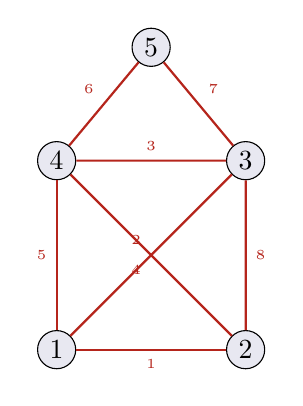
\begin{tikzpicture}[scale=1.2, >=stealth, main node/.style={circle, draw, fill=MidnightBlue!10, inner sep=2pt}]
  \node[main node] (1) at (0,0) {$1$};
  \node[main node] (2) at (2,0) {$2$};
  \node[main node] (3) at (2,2) {$3$};
  \node[main node] (4) at (0,2) {$4$};
  \node[main node] (5) at (1,3.2) {$5$};

  \draw[thick, BrickRed] (1) -- (2) node[midway, below] {\tiny 1};
  \draw[thick, BrickRed] (2) -- (4) node[midway, above left] {\tiny 2};
  \draw[thick, BrickRed] (4) -- (3) node[midway, above] {\tiny 3};
  \draw[thick, BrickRed] (3) -- (1) node[midway, below left] {\tiny 4};
  \draw[thick, BrickRed] (1) -- (4) node[midway, left] {\tiny 5};
  \draw[thick, BrickRed] (4) -- (5) node[midway, above left] {\tiny 6};
  \draw[thick, BrickRed] (5) -- (3) node[midway, above right] {\tiny 7};
  \draw[thick, BrickRed] (3) -- (2) node[midway, right] {\tiny 8};
\end{tikzpicture}
\end{center}

\begin{explanation-of-steps}[Eulerweg beim Haus vom Nikolaus]
Das Haus vom Nikolaus ist ein Graph mit $5$ Knoten und $8$ Kanten. Die Knoten $1$ und $2$ haben jeweils den ungeraden Grad $3$, während die Knoten $3, 4, 5$ den geraden Grad $4$ bzw. $2$ besitzen. Daher existiert ein \emph{offener Eulerweg} mit Start in Knoten $1$ (oder $2$) und Ende in Knoten $2$ (oder $1$).
\end{explanation-of-steps}
\end{math-stroke}

\subsection{Formalisierung und Grundbegriffe}

\begin{spoken-clean}[00:13:00 - 00:14:08]
Genau, aber machen wir das Ganze vielleicht etwas systematischer und definieren das alles sauber. Ich habe jetzt einen Teil der heutigen Vorlesung auf Beamer vorbereitet. Mache ich normalerweise nicht, aber wenn man so viele Definitionen hat, die alle sehr einfach sind, dann ist das etwas mühsam, die alle an die Tafel zu schreiben, man braucht viel Zeit. Schauen wir uns das also auf dem Beamer an. \inlinemetanote{schaltet Beamer ein}

Sehen Sie das gut so? Gut.

Also, was ist ein Graph? Ein Graph ist einfach eine Menge $V$ von sogenannten Knoten zusammen mit einer Teilmenge $E \subseteq V \times V$ oder mehreren Teilmengen $E_0, \dots, E_k \subseteq V \times V$, den sogenannten Kanten. Wir schreiben $G = (V, E)$ respektive $G = (V, E_0, \dots, E_k)$.
\end{spoken-clean}

\begin{math-stroke}
\begin{definition}[Graph]\label[definition]{def:graph-grundbegriff}
Ein \newterm{Graph} ist ein Paar $G = (V, E)$, bestehend aus einer nichtleeren Menge $V$ von \newterm{Knoten} (Vertices) und einer Teilmenge $E \subseteq V \times V$ von \newterm{Kanten} (Edges). 

Falls mehrere Kantenrelationen vorliegen, schreibt man $G = (V, E_0, \dots, E_k)$ mit $E_0, \dots, E_k \subseteq V \times V$.
\end{definition}
\end{math-stroke}

\begin{spoken-clean}[00:14:08 - 00:16:00]
Wir haben $V$, einfach eine Menge --- $V$ auf Englisch ist \qt{vertices}, deswegen $V$. Und jetzt schauen wir $V \times V$ an: Das sind wirklich die geordneten Tupel von Paaren von Knoten, und das sind unsere Kanten. So können wir uns das vorstellen: Nehmen wir zum Beispiel diese hier. Wir können sagen, wir haben hier die Knoten $1, 2, 3, 4$.

Und jetzt können wir sagen: Okay, zwischen den zweien machen wir eine Kante. Das ist einfach die Kante gegeben durch $1$ und $4$. Das geht jetzt aber von $1$ nach $4$, wenn wir sagen, das ist die Kante $\langle 1, 4 \rangle$. Dann können wir hier zum Beispiel eine Kante von $4$ nach $3$ machen, also $\langle 4, 3 \rangle$, und hier von $3$ nach $2$, also $\langle 3, 2 \rangle$. Aber wir können jetzt hier nicht zwei Kanten von $4$ nach $3$ machen, weil es nur ein geordnetes Tupel von $4$ nach $3$ gibt.

Okay, das ist schon ein bisschen eine Sache, aber so sieht jetzt einmal mit dieser Definition ein Graph aus. Wir haben einfach Knoten, und dann schauen wir uns Kanten an, die zwischen diesen Knoten liegen.
\end{spoken-clean}

\begin{math-stroke}[Geordnete Kantenpaare (Gerichteter Graph)]
Sei $V = \{1, 2, 3, 4\}$ die Knotenmenge. Eine gerichtete Kantenmenge als Teilmenge des kartesischen Produkts $E \subseteq V \times V$ ist z.\,B.:
\[
E = \bigl\{ \langle 1, 4 \rangle, \langle 4, 3 \rangle, \langle 3, 2 \rangle \bigr\}.
\]

\begin{center}
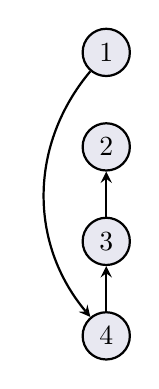
\begin{tikzpicture}[scale=1.2, ->, >=stealth, thick, node/.style={circle, draw, fill=MidnightBlue!10, inner sep=0pt, minimum size=6mm}]
  \node[node] (n1) at (0, 3) {$1$};
  \node[node] (n2) at (0, 2) {$2$};
  \node[node] (n3) at (0, 1) {$3$};
  \node[node] (n4) at (0, 0) {$4$};

  \path
    (n1) edge[bend right=40] (n4)
    (n4) edge (n3)
    (n3) edge (n2);
\end{tikzpicture}
\end{center}
\end{math-stroke}

\begin{spoken-clean}[00:16:00 - 00:17:26]
Gut, jetzt kommt da noch etwas... Ah, hier gibt es noch ein bisschen Terminologie: Wir sagen, zwei Knoten $x, y \in V$ heißen adjazent, falls $(x, y) \in E$. Sie liegen nebeneinander, etwas snobistisch ausgedrückt.

Das Nächste ist ein bisschen verwirrend --- oder auch nicht verwirrend: Wir sagen, falls $E$ symmetrisch ist --- also $E$ kann man ja als ein Relationssymbol auffassen ---: Wir sagen jetzt, ein Graph $G = (V, E)$ ist ungerichtet, falls $E$ symmetrisch ist, d.\,h. falls gilt: $(x, y) \in E$ genau dann, wenn $(y, x) \in E$. In diesem Fall identifizieren wir $(x, y)$ mit $(y, x)$ und schreiben $\{x, y\} \in E$.
\end{spoken-clean}

\begin{math-stroke}
\begin{definition}[Adjazenz und Ungerichteter Graph]\label[definition]{def:adjazenz-ungerichtet}
\begin{itemize}
    \item \textbf{Adjazenz:} Zwei Knoten $x, y \in V$ heißen \newterm{adjazent}, falls $(x, y) \in E$.
    \item \textbf{Ungerichteter Graph:} Ein Graph $G = (V, E)$ heißt \newterm{ungerichtet}, falls die Relation $E$ symmetrisch ist, d.\,h.:
    \[
    (x, y) \in E \iff (y, x) \in E.
    \]
    In diesem Fall identifizieren wir das geordnete Paar $(x, y)$ mit $(y, x)$ und schreiben prägnant $\{x, y\} \in E$.
\end{itemize}
\end{definition}
\end{math-stroke}

\begin{didactic-insight}[Formale Reduktion von Kanten]
Das \qt{Identifizieren} von $(x, y)$ und $(y, x)$ zu der Menge $\{x, y\}$ ist ein informeller, aber in der Graphentheorie allgegenwärtiger Schritt. Formal bedeutet dies, dass wir die Kantenmenge $E$ nicht mehr als Teilmenge des kartesischen Produkts $V \times V$ betrachten, sondern als Menge von $1$- und $2$-elementigen Teilmengen von $V$ (also als Teilmenge von $\mathcal{P}(V)$). Diese formale Substitution vereinfacht die Notation drastisch, da die Reihenfolge der Knoten irrelevant wird.
\end{didactic-insight}

\begin{spoken-clean}[00:17:26 - 00:20:32]
Ein ungerichteter Graph ist eigentlich wie ein gerichteter Graph, aber man darf sich von dieser Unterscheidung nicht zu sehr verwirren lassen. Das ist einfach der Einfachheit halber.

Im Königsberger Brückenproblem darf man natürlich in beide Richtungen laufen, also sowohl von hier nach hier laufen als auch von hier nach hier. Dann würden wir ganz korrekt sagen: Okay, dann haben wir zwei Kanten, eine, die in diese Richtung geht, und eine, die in diese Richtung geht. Und auch hier haben wir eine, die hierhin geht, und eine, die wieder zurückgeht --- wie eine Brücke mit Gegenverkehr. Und anstatt dass wir alle Kanten doppelt hinzeichnen, was etwas mühsam ist, sagen wir einfach: Okay, wir schreiben die nur einfach hin, dafür darf man in beide Richtungen laufen.
\end{spoken-clean}

\begin{student-interaction}[Studentenfrage]
Macht das nicht eigentlich Eulers Argument kaputt? Weil, wenn man bei einem ungerichteten Weg hin- und zurücklaufen kann, also... man muss ja irgendwie codieren, dass man ihn nur einmal benutzen darf.
\end{student-interaction}

\begin{spoken-clean}[00:20:32 - 00:21:12]
Nein, jetzt haben wir jede Brücke nur noch einmal. Aber es sind ja eigentlich ungerichtete Kanten, das heißt, wir identifizieren die beiden Richtungen und haben nur noch eine ungerichtete Kante pro Brücke.
\end{spoken-clean}

\begin{student-interaction}[Studentenfrage]
Und was ist mit $E_0$ und $E_1$?
\end{student-interaction}

\begin{spoken-clean}[00:21:12 - 00:22:55]
Ah, einfach damit wir hier zwei Brücken haben können, ja genau! Wir haben da noch eine vergessen, oder? \inlinemetanote{korrigiert die Skizze an der Tafel} $\{1, 2\}$ und $\{1, 3\}$ haben wir noch vergessen. Weil dieser hier ist nicht derselbe wie dieser hier.

Einfach so viel noch zur Definition. Es ist ein bisschen mühsam, wenn man die Definition so sieht, aber es ist genau das, was Sie sich unter einem Graphen vorstellen.
\end{spoken-clean}

\begin{math-stroke}[Formalisierung des Königsberger Multigraphen]
Für den Königsberger Graph mit $V = \{1, 2, 3, 4\}$ wählen wir zwei Kantenmengen $E_0, E_1$, um Mehrfachbrücken abzubilden:
\begin{align*}
E_0 &= \bigl\{ \{1, 4\}, \{3, 4\}, \{2, 3\}, \{1, 2\} \bigr\}, \\
E_1 &= \bigl\{ \{3, 4\}, \{2, 3\}, \{1, 3\} \bigr\}.
\end{align*}
\end{math-stroke}

\begin{spoken-clean}[00:22:55 - 00:25:32]
Gut, das ist für einen ungerichteten Graphen.

Dann sagen wir: Ein Graph heißt gerichtet oder ein Digraph, falls er nicht ungerichtet ist. Okay... was heißt \qt{Nicht-Definitionen} halt... Und oft, anstatt gerichtet, sagt man auch ein Digraph. Weshalb Digraph? Halt eben, weil es zwei verschiedene Richtungen gibt, quasi.

Und das hängt sehr stark vom Gebiet ab, wo Sie arbeiten. Ich würde fast sagen, meistens verwendet man öfters ungerichtete Graphen als gerichtete Graphen.

Dann: Eine Kante von der Form $(x, x) \in E$ heißt Schlinge. Es spricht also nichts dagegen, dass man hier eine Kante der Form $(x, x)$ hat. Das ist dann einfach eine solche Kante, und diese heißen Schlingen. Wenn es ein gerichteter Graph ist, würde man das einfach so bezeichnen. Eine Schlinge hat keine Richtung.

Und entsprechend heißt ein Graph $G$ schlingenfrei, falls er keine Schlingen besitzt.

Falls $G = (V, E_0, \dots, E_k)$, so kann es zwischen zwei Knoten mehrere Kanten geben, die verschieden sind. Solche Kanten heißen Mehrfachkanten.

Und ein Graph ohne Schlingen und ohne Mehrfachkanten heißt schlicht. Ein schlichter Graph ist einfach ein Graph, wo man das nicht hat und Mehrfachkanten auch nicht haben kann.
\end{spoken-clean}

\begin{math-stroke}
\begin{definition}[Digraph, Schlinge, Mehrfachkanten und Schlichter Graph]\label[definition]{def:graphen-klassifikation}
\begin{itemize}
    \item \textbf{Digraph (Gerichteter Graph):} Ein Graph $G$ heißt \newterm{gerichtet} oder \newterm{Digraph}, falls er nicht ungerichtet ist.
    \item \textbf{Schlinge:} Eine Kante der Form $(x, x) \in E$ heißt \newterm{Schlinge}. Ein Graph heißt \newterm{schlingenfrei}, falls er keine Schlingen besitzt.
    \item \textbf{Mehrfachkanten:} Falls $G = (V, E_0, \dots, E_k)$, so kann es zwischen zwei Knoten mehrere verschiedene Kanten geben. Solche Kanten heißen \newterm{Mehrfachkanten}.
    \item \textbf{Schlichter Graph:} Ein Graph ohne Schlingen und ohne Mehrfachkanten heißt \newterm{schlicht}.
\end{itemize}
\end{definition}

\textbf{Beispiele für Schlichtheit an der Tafel:}
\begin{center}
\setlength{\tabcolsep}{16pt}
\begin{tabular}{c c}
    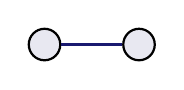
\begin{tikzpicture}[scale=0.8, thick]
        \node[circle, draw, fill=MidnightBlue!10, inner sep=0pt, minimum size=4mm] (A) at (0,0) {};
        \node[circle, draw, fill=MidnightBlue!10, inner sep=0pt, minimum size=4mm] (B) at (1.5,0) {};
        \draw[MidnightBlue] (A) -- (B);
    \end{tikzpicture} &
    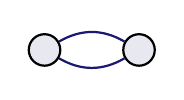
\begin{tikzpicture}[scale=0.8, thick]
        \node[circle, draw, fill=MidnightBlue!10, inner sep=0pt, minimum size=4mm] (A) at (0,0) {};
        \node[circle, draw, fill=MidnightBlue!10, inner sep=0pt, minimum size=4mm] (B) at (1.5,0) {};
        \draw[MidnightBlue] (A) to[bend left=30] (B);
        \draw[MidnightBlue] (A) to[bend right=30] (B);
    \end{tikzpicture} \\[4pt]
    \text{schlicht} & \text{nicht schlicht (Mehrfachkante)} \\[12pt]
    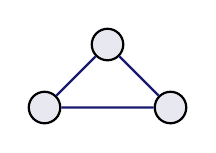
\begin{tikzpicture}[scale=0.8, thick]
        \node[circle, draw, fill=MidnightBlue!10, inner sep=0pt, minimum size=4mm] (A) at (0,0) {};
        \node[circle, draw, fill=MidnightBlue!10, inner sep=0pt, minimum size=4mm] (B) at (1,1) {};
        \node[circle, draw, fill=MidnightBlue!10, inner sep=0pt, minimum size=4mm] (C) at (2,0) {};
        \draw[MidnightBlue] (A) -- (B) -- (C) -- (A);
    \end{tikzpicture} &
    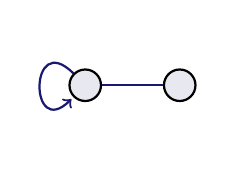
\begin{tikzpicture}[scale=0.8, thick]
        \node[circle, draw, fill=MidnightBlue!10, inner sep=0pt, minimum size=4mm] (A) at (0,0) {};
        \node[circle, draw, fill=MidnightBlue!10, inner sep=0pt, minimum size=4mm] (B) at (1.5,0) {};
        \draw[MidnightBlue] (A) -- (B);
        \path (A) edge[out=135, in=225, distance=1cm, loop, MidnightBlue] (A);
    \end{tikzpicture} \\[4pt]
    \text{schlicht} & \text{nicht schlicht (Schlinge)}
\end{tabular}
\end{center}
\end{math-stroke}

\section{Die Adjazenzmatrix}

\subsection{Definition und Beispiele der Adjazenzmatrix}

\begin{spoken-clean}[00:25:32 - 00:28:49]
Gut, dann die nächste Definition: Sei $G = (V, E)$ ein endlicher Graph, d.\,h. $|V|$ ist endlich. Die Adjazenzmatrix $A(G) = (a_{ij})$ ist eine $n \times n$-Matrix, wobei $V = \{v_1, \dots, v_n\}$, gegeben durch:
\[
a_{ij} = \begin{cases} 1 & \text{falls } (v_i, v_j) \in E, \\ 0 & \text{sonst.} \end{cases}
\]
Für $V = \{v_1, \dots, v_n\}$ nummerieren wir die Knoten durch und sagen: $a_{ij}$ ist $1$, falls es eine Kante von $v_i$ nach $v_j$ gibt, und $0$ sonst.

So ein Graph mit nur einer Kantenrelation ist also einfach durch eine Adjazenzmatrix gegeben, in der es immer Einsen und Nullen gibt.
\end{spoken-clean}

\begin{spoken-clean}[00:28:49 - 00:30:10]
Machen wir ein Beispiel: Nehmen wir den Graphen mit $V = \{1, 2, 3, 4\}$, und wir haben hier eine Kante von $1$ nach $2$, eine von $2$ nach $3$, eine von $3$ nach $4$ und eine von $4$ nach $1$.

Was wäre die Adjazenzmatrix von diesem Graphen? Von $1$ nach $1$ gibt es nichts. Von $1$ nach $2$ gibt es etwas, und sonst wieder nichts. Dann von $2$ nach... das Einzige von $2$ aus gibt es eine Kante nach $3$, aber sonst nichts. Von $3$ gibt es eine nach $4$, aber sonst nichts. Und von $4$ gibt es eine nach $1$.
\end{spoken-clean}

\begin{math-stroke}
\begin{definition}[Adjazenzmatrix]\label[definition]{def:adjazenzmatrix}
Sei $G = (V, E)$ ein endlicher Graph mit nummerierter Knotenmenge $V = \{v_1, \dots, v_n\}$. Die \newterm{Adjazenzmatrix} $A(G) = (a_{ij}) \in M_{n \times n}(\mathbb{R})$ ist definiert durch:
\begin{equation}\label{eq:adjazenzmatrix-def}
a_{ij} := \begin{cases}
1 & \text{falls } (v_i, v_j) \in E, \\
0 & \text{sonst.}
\end{cases}
\end{equation}
\end{definition}

\begin{example}[Adjazenzmatrix eines gerichteten 4-Zyklus]
\label[example]{ex:adjazenzmatrix-4-zyklus}
Sei $V = \{1, 2, 3, 4\}$ und $E = \{ (1,2), (2,3), (3,4), (4,1) \}$.

\begin{center}
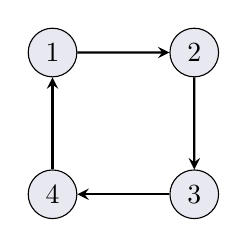
\begin{tikzpicture}[scale=1.2, >=stealth, node distance=1.8cm]
  \node[circle, draw, fill=MidnightBlue!10] (n1) at (0, 1.5) {$1$};
  \node[circle, draw, fill=MidnightBlue!10] (n2) at (1.5, 1.5) {$2$};
  \node[circle, draw, fill=MidnightBlue!10] (n3) at (1.5, 0) {$3$};
  \node[circle, draw, fill=MidnightBlue!10] (n4) at (0, 0) {$4$};

  \draw[->, thick] (n1) -- (n2);
  \draw[->, thick] (n2) -- (n3);
  \draw[->, thick] (n3) -- (n4);
  \draw[->, thick] (n4) -- (n1);
\end{tikzpicture}
\end{center}

Die zugehörige Adjazenzmatrix lautet:
\[
A(G) = \begin{pmatrix}
0 & 1 & 0 & 0 \\
0 & 0 & 1 & 0 \\
0 & 0 & 0 & 1 \\
1 & 0 & 0 & 0
\end{pmatrix}.
\]
\end{example}
\end{math-stroke}

\begin{spoken-clean}[00:30:10 - 00:33:00]
Okay, und dann ist noch die Frage, falls wir mehrere Kanten zwischen zwei Knoten haben: Wenn wir also in dem anderen Fall sind, dann ist das analog. Dann zählen wir einfach: Wie viele gibt es dazwischen?

Okay, wenn wir $G$ schreiben als $V$ mit $E_1$ bis $E_k$, also verschiedene Kantenmengen haben, aber auch $|V|$ endlich ist: In dem Fall definieren wir den Graphen $G_\ell$ als den Graphen mit Knotenmenge $V$ und nehmen jetzt einfach nur die Relation $E_\ell$ dazu.

Und dann definieren wir die Adjazenzmatrix von $G$ als die Summe aller Adjazenzmatrizen von $G_\ell$. Das heißt mit anderen Worten: Im Prinzip zählen wir einfach, wie viele Kanten vom Knoten $i$ zum Knoten $j$ gehen. Okay?

Machen wir noch ein Beispiel, was weiß ich: Nehmen wir $1, 2$, und wir haben hier zwei Kanten. Wenn wir das $G$ nennen, wir haben eine Kante so und eine Kante so. Dann ist die entsprechende Adjazenzmatrix von $G$: Von $1$ nach $1$ gibt es keinen, von $1$ nach $2$ gibt es $2$, von $2$ nach $1$ gibt es keinen und von $2$ nach $2$ gibt es auch keinen. Okay? Und das ist einfach... ja, wie wir sehen, ist das einfach:
\[
\begin{pmatrix} 0 & 2 \\ 0 & 0 \end{pmatrix} = \begin{pmatrix} 0 & 1 \\ 0 & 0 \end{pmatrix} + \begin{pmatrix} 0 & 1 \\ 0 & 0 \end{pmatrix}.
\]
\end{spoken-clean}

\begin{math-stroke}[Adjazenzmatrix für Multigraphen]
Falls $G = (V, E_1, \dots, E_k)$ ein Multigraph mit $|V|$ endlich ist, setzt man $G_\ell := (V, E_\ell)$ für $\ell \in \{1, \dots, k\}$ und definiert:
\begin{equation}\label{eq:adjazenzmatrix-multigraph-summe}
A(G) := \sum_{\ell=1}^k A(G_\ell).
\end{equation}

\begin{example}[Parallele gerichtete Kanten]
Sei $G$ der Graph auf $V = \{1, 2\}$ mit zwei parallelen gerichteten Kanten von $1$ nach $2$:

\begin{center}
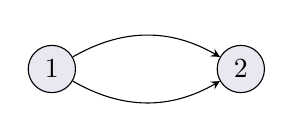
\begin{tikzpicture}[scale=1.2, ->, >=stealth, node/.style={circle, draw, fill=MidnightBlue!10, inner sep=0pt, minimum size=6mm}]
  \node[node] (n1) at (0, 0) {$1$};
  \node[node] (n2) at (2, 0) {$2$};

  \path
    (n1) edge[bend left=30] (n2)
    (n1) edge[bend right=30] (n2);
\end{tikzpicture}
\end{center}

Die Adjazenzmatrix berechnet sich zu:
\[
A(G) = \begin{pmatrix} 0 & 2 \\ 0 & 0 \end{pmatrix} = \begin{pmatrix} 0 & 1 \\ 0 & 0 \end{pmatrix} + \begin{pmatrix} 0 & 1 \\ 0 & 0 \end{pmatrix}.
\]
\end{example}
\end{math-stroke}

\begin{spoken-clean}[00:33:00 - 00:34:51]
Schauen wir uns hier noch ein etwas komplizierteres Beispiel an, das ist auch im Skript. Wenn wir diesen Graphen hier anschauen:

Okay, da haben wir sechs Knoten. Das heißt, was ist da die Adjazenzmatrix? Von $1$ nach $1$ gibt es keine Kanten, das heißt, da ist $0$. Von $1$ nach $2$ gibt es eine. Von $1$ nach $3$ gibt es keine. Dann gibt es auch keine nach $4$, es gibt aber noch eine nach $5$ und eine nach $6$.

Von $2$ nach $1$ gibt es eine. Von $2$ nach $2$ gibt es keine. Von $2$ nach $3$ gibt es keine. Von $2$ nach $4$ gibt es keine. Von $2$ nach $5$ gibt es eine. Von $2$ nach $6$ gibt es keine.

Von $3$ nach $1$ gibt es keine. Von $3$ nach $2$... ja, müssen wir jetzt nicht alles durchmachen. Hier gibt es noch eine von $3$ nach $3$, von $3$ nach $4$ gibt es $2$... Okay, und so weiter. Das müssen wir nicht mehr hinschreiben. Ist das klar? Gut.
\end{spoken-clean}

\begin{math-stroke}[Komplexeres Beispiel eines gerichteten Multigraphen]
\begin{meta-note}[Projizierte Folie: Beispielgraph]
Die Folie zeigt einen gerichteten Graphen mit $6$ Knoten $\{1, 2, 3, 4, 5, 6\}$, einer Schlinge an Knoten $3$, sowie Doppel Kanten zwischen $3$ und $4$ bzw. $5$ und $4$.
\end{meta-note}

\begin{center}
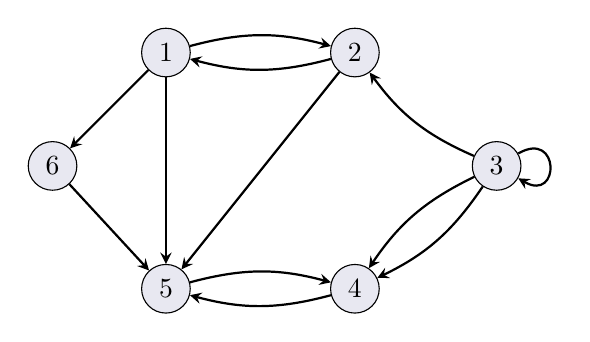
\begin{tikzpicture}[scale=1.2, ->, >=stealth, node/.style={circle, draw, fill=MidnightBlue!10, font=\bfseries}]
  \node[node] (n1) at (0, 2) {$1$};
  \node[node] (n2) at (2, 2) {$2$};
  \node[node] (n3) at (3.5, 0.8) {$3$};
  \node[node] (n4) at (2, -0.5) {$4$};
  \node[node] (n5) at (0, -0.5) {$5$};
  \node[node] (n6) at (-1.2, 0.8) {$6$};

  \draw[thick] (n1) to[bend left=15] (n2);
  \draw[thick] (n2) to[bend left=15] (n1);
  \draw[thick] (n1) -- (n5);
  \draw[thick] (n1) -- (n6);
  \draw[thick] (n2) -- (n5);
  \draw[thick] (n6) -- (n5);
  \draw[thick] (n3) to[bend left=15] (n2);
  \draw[thick] (n3) to[out=30, in=-30, looseness=5] (n3);
  \draw[thick] (n3) to[bend left=15] (n4);
  \draw[thick] (n3) to[bend right=15] (n4);
  \draw[thick] (n5) to[bend left=15] (n4);
  \draw[thick] (n4) to[bend left=15] (n5);
\end{tikzpicture}
\end{center}

Die zugehörige $6 \times 6$-Adjazenzmatrix lautet:
\[
A(G) = \begin{pmatrix}
0 & 1 & 0 & 0 & 1 & 1 \\
1 & 0 & 0 & 0 & 1 & 0 \\
0 & 1 & 1 & 2 & 0 & 0 \\
\vdots & & & & & \vdots
\end{pmatrix}.
\]
\end{math-stroke}

\begin{spoken-clean}[00:34:51 - 00:37:48]
Können wir vielleicht noch kurz den Graphen vom Königsberger Brückenproblem durchrechnen. Wie hatten wir die Nummerierung? $1, 2, 3, 4$, und da hatten wir so etwas. Das war $G$. Was ist jetzt da die Adjazenzmatrix?

Okay, das ist jetzt ein ungerichteter Graph. Aber dem können wir doch auch eine Adjazenzmatrix zuordnen. Und das ist genau dieselbe, wie wenn wir sagen: Die Kante von $1$ nach $2$ ist jetzt auch eine Kante von $2$ nach $1$. Und dann passt alles wieder.

Das heißt, hier haben wir eine $4 \times 4$-Matrix: Von $1$ nach $1$ gibt es keine, von $1$ nach $2$ gibt es $2$, von $1$ nach $3$ keine, von $1$ nach $4$ eine. Von $2$ nach $1$ gibt es $2$, von $2$ nach $2$ keine, von $2$ nach $3$ $2$, von $2$ nach $4$ eine. Von $3$ nach $1$ gibt es keine, von $3$ nach $2$ gibt es $2$, von $3$ nach $3$ gibt es keine, von $3$ nach $4$ gibt es eine. Und von $4$ gibt es eine nach $1$, eine nach $2$, eine nach $3$, und nach $4$ gibt es keine.

Okay, macht auch Sinn. Auch für ungerichtete Graphen ist das sehr klar.

Okay, alles klar bei der Adjazenzmatrix? Wenn man die Adjazenzmatrix hat, dann hat man eigentlich alle wesentlichen Informationen. Und wie Sie wissen, schaut man sich ja immer gerne Matrizen an, weil man die lineare Algebra gut verstanden hat. Sie haben vielleicht schon ein bisschen bemerkt: Ein Großteil der Mathematik besteht eigentlich darin, alles auf die lineare Algebra zurückzuführen.

Man hat die meisten Sachen nicht verstanden; eine der wenigen Sachen, die man gut verstanden hat, ist die lineare Algebra. Deswegen hat man im ersten Jahr schon einen ganzen Kurs darüber. In der Analysis geht es eigentlich darum, irgendetwas, was man nicht verstanden hat, durch lineare Abbildungen zu approximieren, und das hat man dann verstanden. Und Sie werden auch in anderen Bereichen der Mathematik sehen: Man hat irgendetwas, was man nicht verstanden hat, man versucht Vektorräume dazuzuordnen, und die hat man verstanden, und dann kann man das Problem lösen. Ja, Mathematik besteht vielleicht daraus, Probleme auf lineare Algebra zu reduzieren, und dann kann man die Probleme lösen.
\end{spoken-clean}

\begin{math-stroke}[Adjazenzmatrix des Königsberger Graphen]
Für den ungerichteten Königsberger Multigraphen $G$ mit $V = \{1, 2, 3, 4\}$:

\begin{center}
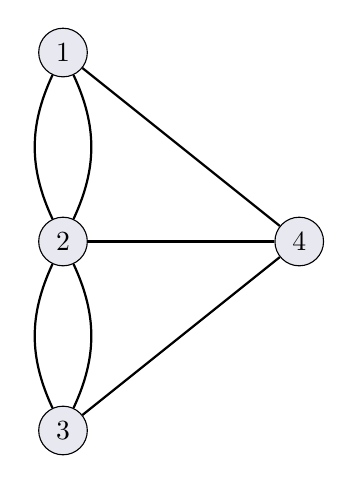
\begin{tikzpicture}[scale=1.2, >=stealth, node/.style={circle, draw, fill=MidnightBlue!10, font=\bfseries}]
  \node[node] (n1) at (0, 2) {$1$};
  \node[node] (n2) at (0, 0) {$2$};
  \node[node] (n3) at (0, -2) {$3$};
  \node[node] (n4) at (2.5, 0) {$4$};

  \draw[thick] (n1) to[bend left=25] (n2);
  \draw[thick] (n1) to[bend right=25] (n2);
  \draw[thick] (n2) to[bend left=25] (n3);
  \draw[thick] (n2) to[bend right=25] (n3);
  \draw[thick] (n1) -- (n4);
  \draw[thick] (n2) -- (n4);
  \draw[thick] (n3) -- (n4);
\end{tikzpicture}
\end{center}

erhält man die symmetrische $4 \times 4$-Adjazenzmatrix:
\[
A(G) = \begin{pmatrix}
0 & 2 & 0 & 1 \\
2 & 0 & 2 & 1 \\
0 & 2 & 0 & 1 \\
1 & 1 & 1 & 0
\end{pmatrix}.
\]
\end{math-stroke}

\begin{didactic-insight}[Die Brücke zur Linearen Algebra: Warum Matrizen in der Graphentheorie?]
Die Einführung der Adjazenzmatrix ist weit mehr als eine bloße tabellarische Auflistung von Kanten. Sie schlägt eine fundamentale Brücke zur Linearen Algebra:
\begin{itemize}
    \item \textbf{Pfadzählung:} Ein zentrales Resultat besagt, dass der Eintrag $(i,j)$ der $k$-ten Potenz der Adjazenzmatrix, also $A(G)^k$, exakt der Anzahl aller gerichteten Kantenfolgen der Länge $k$ vom Knoten $v_i$ zum Knoten $v_j$ entspricht.
    \item \textbf{Spektrale Graphentheorie:} Die Eigenwerte der Adjazenzmatrix (das sogenannte Spektrum des Graphen) kodieren tiefgreifende strukturelle Eigenschaften des Graphen, wie etwa seine Konnektivität, chromatische Zahl oder ob er bipartit ist.
\end{itemize}
\end{didactic-insight}

\subsection{Eigenschaften der Adjazenzmatrix}

\begin{spoken-clean}[00:37:48 - 00:39:45]
Vielleicht noch ein paar Bemerkungen, die relativ einfach aus der Definition folgen: Wenn $A(G) = (a_{ij})$ die Adjazenzmatrix ist, dann sind die $a_{ij}$ alle größer gleich $0$ und ganze Zahlen --- in $\omega$, wenn Sie wollen. Okay, das heißt, es ist eine ganzzahlige Matrix aus nicht-negativen Zahlen.

Jetzt, was können wir über Schlingenfreiheit sagen? $G$ ist schlingenfrei genau dann, wenn $a_{ii} = 0$ gilt für alle $i$. Okay, das ist, wenn es keine Kante von einem Knoten zu sich selbst gibt. Wenn aber $a_{ii} = 0$ für alle $i$ gilt, dann folgt daraus, dass die Spur dieser Matrix $0$ ist.

Und wenn die Spur der Adjazenzmatrix $0$ ist, das heißt, die Summe all dieser $a_{ii}$ ist $0$ --- aber die $a_{ii}$ sind ja alle nicht-negativ ---, dann ist die einzige Möglichkeit, dass die Spur $0$ sein kann, dass $a_{ii} = 0$ für alle $i$ ist. Das heißt: $G$ ist schlingenfrei genau dann, wenn die Spur der Adjazenzmatrix $0$ ist. Man sieht also an der Spur der Matrix direkt, ob der Graph schlingenfrei ist oder nicht.
\end{spoken-clean}

\begin{math-stroke}
\begin{remark}[Eigenschaften der Eintragsmatrix]
Sei $A(G) = (a_{ij})$ die Adjazenzmatrix eines Graphen $G$:
\begin{enumerate}[label=\textbf{(\roman*)}]
    \item $a_{ij} \ge 0$ und $a_{ij} \in \mathbb{N}_0$ für alle $i, j$ (nicht-negative Ganzzahligkeit).
    \item $G$ ist schlingenfrei genau dann, wenn $a_{ii} = 0$ für alle $i$.
    \item Da $a_{ii} \ge 0$, gilt:
    \[
    G \text{ ist schlingenfrei} \iff \operatorname{Spur}(A(G)) = \sum_{i=1}^n a_{ii} = 0.
    \]
\end{enumerate}
\end{remark}
\end{math-stroke}

\begin{spoken-clean}[00:39:45 - 00:41:27]
Als Nächstes: Wie sieht man an der Adjazenzmatrix, ob der Graph ungerichtet ist oder nicht?

Noch eine weitere Bemerkung: Der Graph $G$ ist ungerichtet genau dann, wenn $A(G)$... ja?
\end{spoken-clean}

\begin{student-interaction}[Studentenantwort]
...wenn sie symmetrisch ist.
\end{student-interaction}

\begin{spoken-clean}[00:41:27 - 00:41:30]
Genau, wenn sie symmetrisch ist. Ist klar, $A(G)$ ist dann symmetrisch. Okay, das heißt... ja, genau, das macht Sinn.

Das heißt, $G$ ist ungerichtet, wenn für jede Kante $(v_1, v_2)$ auch $(v_2, v_1)$ wieder eine Kante ist; das ist aber äquivalent dazu, dass die Matrix symmetrisch ist.
\end{spoken-clean}

\begin{math-stroke}
\begin{proposition}[Symmetrie der Adjazenzmatrix]\label[proposition]{prop:adjazenzmatrix-symmetrie}
Ein Graph $G$ ist ungerichtet genau dann, wenn seine Adjazenzmatrix $A(G)$ symmetrisch ist:
\[
G \text{ ungerichtet} \iff A(G) = A(G)^T.
\]
\end{proposition}
\end{math-stroke}

\section{Knotengrad in Graphen}
% Old section name: 3.3 Knotengrad in Gerichteten Graphen (Halbgrade) & 3.4 Knotengrad in Ungerichteten Graphen

\subsection{Knotengrad in Gerichteten Graphen (Halbgrade)}

\begin{spoken-clean}[00:41:30 - 00:43:00]
Okay, dann machen wir noch ein paar weitere Definitionen an der Tafel, und danach machen wir Pause.

Folgende Definition: Sei $G = (V, E)$ ein Digraph, also ein gerichteter Graph. Für einen Knoten $x$ von $G$ definieren wir zuerst einmal $\Gamma^+(x)$. Das definieren wir als alle Knoten $y \in V$, sodass $(x, y)$ eine Kante ist. Okay, das sind quasi alle... Wenn Sie hier $x$ haben, schauen wir alle $y$ an, sodass es hier eine Kante von $x$ nach $y$ gibt. Das ist diese Menge hier.

Und analog ist $\Gamma^-(x)$ die Menge aller $y \in V$, sodass $(y, x)$ wieder eine Kante ist. Okay, das heißt, das sind alle $y$, sodass es eine Kante von $y$ nach $x$ gibt.
\end{spoken-clean}

\begin{math-stroke}
\begin{definition}[Nachbarschaftsmengen im Digraphen]\label[definition]{def:digraph-nachbarschaft}
Sei $G = (V, E)$ ein gerichteter Graph (Digraph) und $x \in V$ ein Knoten.
\begin{itemize}
    \item \textbf{Positiver Nachbereich (Ausgangsnachbarn):}
    \[
    \Gamma^+(x) := \bigl\{ y \in V \big| (x, y) \in E \bigr\}
    \]
    \item \textbf{Negativer Nachbereich (Eingangsnachbarn):}
    \[
    \Gamma^-(x) := \bigl\{ y \in V \big| (y, x) \in E \bigr\}
    \]
\end{itemize}
\end{definition}
\end{math-stroke}

\begin{spoken-clean}[00:43:00 - 00:45:02]
Gut, und dann definieren wir den positiven Halbgrad $\operatorname{deg}^+(x)$ als die Kardinalität von $\Gamma^+(x)$. Das ist der positive Halbgrad. Und entsprechend den negativen Halbgrad als die Kardinalität von $\Gamma^-(x)$ --- negativer Halbgrad.

Und dann werden wir den Grad von $x$ definieren als die Summe vom positiven und dem negativen Halbgrad. Das ist genau die Anzahl der Kanten, die von $x$ ausgehen oder reingehen.

Wir müssen noch schauen: Noch kurz ein Beispiel, bevor wir Pause machen. Wenn $x$ von dieser Form ist: $x$, und es gibt hier einfach eine Schlinge --- was ist dann der Grad von $x$? Ja?
\end{spoken-clean}

\begin{student-interaction}[Studentenantwort]
2.
\end{student-interaction}

\begin{spoken-clean}[00:45:02 - 00:45:03]
2, genau! Weil wir haben hier: Einmal geht es raus und einmal geht es rein, es wird zweimal gezählt. Macht auch Sinn, ist das, was wir gerne hätten. Gut.

Ja, dann machen wir Pause.
\end{spoken-clean}

\begin{math-stroke}
\begin{definition}[Halbgrade und Grad im Digraphen]\label[definition]{def:digraph-halbgrade}
Sei $G = (V, E)$ ein Digraph und $x \in V$.
\begin{itemize}
    \item \textbf{Positiver Halbgrad (Ausgangsgrad):} $\operatorname{deg}^+(x) := |\Gamma^+(x)|$.
    \item \textbf{Negativer Halbgrad (Eingangsgrad):} $\operatorname{deg}^-(x) := |\Gamma^-(x)|$.
    \item \textbf{Gesamtgrad:} $\operatorname{deg}(x) := \operatorname{deg}^+(x) + \operatorname{deg}^-(x)$.
\end{itemize}
\end{definition}

\begin{example}[Schlinge an einem Knoten]
Besitzt ein Knoten $x$ eine Schlinge $(x, x) \in E$, so gilt $x \in \Gamma^+(x)$ und $x \in \Gamma^-(x)$. Die Schlinge erhöht sowohl $\operatorname{deg}^+(x)$ als auch $\operatorname{deg}^-(x)$ um $1$, womit sie insgesamt mit $2$ zum Gesamtgrad $\operatorname{deg}(x)$ beiträgt.
\end{example}
\end{math-stroke}

\begin{lecture-break}[Vorlesungspause]
Der Dozent kündigt eine kurze Pause an. Das Video wird nach der Pause bei Zeitstempel 00:45:03 fortgesetzt.
\end{lecture-break}

\subsection{Knotengrad in Ungerichteten Graphen}

\begin{spoken-clean}[00:45:03 - 00:47:17]
Wir machen langsam weiter. Wir hatten vor der Pause noch die Definition des Grades für gerichtete Graphen gesehen.

Wenn unser Graph ungerichtet ist, dann definieren wir $\Gamma(x)$ --- da gibt es kein $\Gamma^+$ und $\Gamma^-$ mehr --- als alle $y \in V$, sodass $\{x, y\} \in E$ ist. Und in dem Fall definieren wir jetzt den Grad von $x$ als...

Okay, und damit wir hier das Richtige kriegen: Hier wollen wir einfach wieder wissen, wie viele Kanten von dort ausgehen. Da interessiert uns die Richtung nicht mehr, weil das dasselbe ist. Wenn wir jetzt so einen Graphen haben... ja gut, das ist nicht das beste Beispiel... Wenn wir so etwas haben, einen ungerichteten Graphen, wollen wir einfach, dass dieser Knoten hier Grad $4$ hat. Nämlich einfach die Anzahl aller Kanten, die von hier aus weggehen. Das definieren wir als die Kardinalität von diesem $\Gamma(x)$.

Aber das Problem, das wir jetzt dabei noch ein bisschen haben, ist, wenn wir eine Schlinge haben. Wenn wir so etwas haben, wird das im Moment nur einmal gezählt. Wir hätten aber gerne, dass das hier im ungerichteten Fall Grad $2$ hat. Und deswegen müssen wir eigentlich, wenn es eine Schlinge gibt, die einfach noch dazuzählen. Das ist ein bisschen diese technische Definition im Skript: Das ist die Menge von allen $z \in V$, sodass $z = x$ und $\{x, z\} \in E$. Aber okay, $x$ ist ja gegeben. Das heißt, diese Menge hier besteht entweder aus $\{x\}$ oder sie ist leer. Das heißt, entweder $0$ oder $1$ müssen wir noch dazuzählen.
\end{spoken-clean}

\begin{math-stroke}
\begin{definition}[Nachbarschaft und Grad im ungerichteten Graphen]\label[definition]{def:ungerichtet-grad}
Sei $G = (V, E)$ ein ungerichteter Graph und $x \in V$.
\begin{itemize}
    \item \textbf{Nachbarschaftsmenge:} $\Gamma(x) := \bigl\{ y \in V \big| \{x, y\} \in E \bigr\}$.
    \item \textbf{Knotengrad:} Der \newterm{Grad} $\operatorname{deg}(x)$ zählt die Anzahl der in $x$ inzidenten Kantenenden, wobei Schlingen doppelt gezählt werden:
    \begin{equation}\label{eq:ungerichtet-grad-def}
    \operatorname{deg}(x) := |\Gamma(x)| + \bigl| \{ z \in V \mid z = x \land \{x, z\} \in E \} \bigr|.
    \end{equation}
\end{itemize}
\end{definition}
\end{math-stroke}

\begin{spoken-clean}[00:47:17 - 00:49:17]
Okay, das ist die Definition von Grad für ungerichtete Graphen. Und sowohl für gerichtete als auch für ungerichtete Graphen: Falls unser Graph von der Form $G = (V, E_0, \dots, E_k)$ ist, kann man das wieder genau gleich definieren, aber wir nehmen wieder die Summe von all den Teilgraphen, die wir vorher definiert hatten.

Dann definiert man analog: Der Grad $\operatorname{deg}_G(x)$ ist dann einfach $\operatorname{deg}_{G_0}(x) + \dots + \operatorname{deg}_{G_k}(x)$. Und ähnlich für den positiven Grad $\operatorname{deg}_G^+(x)$...
\end{spoken-clean}

\begin{math-stroke}[Gradbestimmung in Multigraphen]
Falls $G = (V, E_0, \dots, E_k)$ ein Multigraph ist, summiert sich der Grad über alle Kantenrelationen $G_\ell = (V, E_\ell)$:
\begin{align}
\operatorname{deg}_G(x) &:= \sum_{\ell=0}^k \operatorname{deg}_{G_\ell}(x), \label{eq:multigraph-grad-gesamte} \\
\operatorname{deg}_G^+(x) &:= \sum_{\ell=0}^k \operatorname{deg}_{G_\ell}^+(x), \quad \operatorname{deg}_G^-(x) := \sum_{\ell=0}^k \operatorname{deg}_{G_\ell}^-(x). \nonumber
\end{align}
\end{math-stroke}

\section{Spezielle Graphenklassen}

\subsection{Reguläre Graphen}

\begin{spoken-clean}[00:49:17 - 00:51:35]
Okay, klar, das gibt genau das, was man möchte.

Okay, dann machen wir noch die folgende Definition: Ein ungerichteter Graph $G = (V, E)$ heißt regulär vom Grad $r$, falls der Grad von $x$ gleich $r$ ist für alle $x \in V$. Okay, also einfach, falls der Grad überall derselbe ist.

Da vielleicht noch ein paar Beispiele: Dieser Graph hier zum Beispiel ist regulär vom Grad $2$.

Oder wir können zum Beispiel so einen unendlichen Graphen anschauen: Man beginnt zum Beispiel hier, dann lässt man von einem Knoten drei Kanten weggehen, und von jedem dieser Knoten lässt man wieder zwei weggehen, und wieder zwei weggehen... Das geht dann immer so weiter. So ein sogenannter Baum, der ist auch regulär vom Grad $3$.
\end{spoken-clean}

\begin{math-stroke}
\begin{definition}[Regulärer Graph]\label[definition]{def:regulaerer-graph}
Ein ungerichteter Graph $G = (V, E)$ heißt \newterm{regulär} vom Grad $r$ ($r$-regulär), falls jeder Knoten den Grad $r$ besitzt:
\begin{equation}\label{eq:regulaer-def}
\forall x \in V \colon \operatorname{deg}(x) = r.
\end{equation}
\end{definition}

\begin{examples}[Reguläre Graphen]
\label[examples]{exm:regulaere-graphen}
\begin{enumerate}[label=\textbf{(\arabic*)}]
    \item \textbf{Kreisgraph / Quadrat ($\mathbf{C_4}$):} Der Quadratgraph ist $2$-regulär:
    \begin{center}
    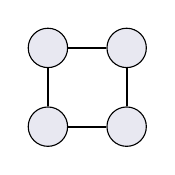
\begin{tikzpicture}[scale=1.0, node/.style={circle, draw, fill=MidnightBlue!10, inner sep=0pt, minimum size=5mm}]
      \node[node] (n1) at (0, 1) {};
      \node[node] (n2) at (1, 1) {};
      \node[node] (n3) at (1, 0) {};
      \node[node] (n4) at (0, 0) {};
      \draw[thick] (n1) -- (n2) -- (n3) -- (n4) -- (n1);
    \end{tikzpicture}
    \end{center}
    \item \textbf{Unendlicher 3-regulärer Baum:} Ein unendlicher Verzweigungsbaum, bei dem von jedem Knoten $3$ Kanten ausgehen, ist $3$-regulär.
\end{enumerate}
\end{examples}
\end{math-stroke}

\subsection{Vollständige Graphen}

\begin{spoken-clean}[00:51:35 - 00:54:44]
Und wir sagen noch: Ein ungerichteter Graph $G = (V, E)$ heißt vollständig, falls für alle $x, y \in V$ mit $x \neq y$ gilt: $\{x, y\} \in E$. Okay, das heißt, falls alle Knoten miteinander verbunden sind, ist der Graph vollständig. Also zum Beispiel so etwas: Hier haben wir drei Knoten, und jeder von diesen Knoten ist noch mit den anderen zwei verbunden.

Okay, und diese Definition... das ist die Definition aus dem Skript, aber in der Regel möchte man eigentlich keine Schlingen im vollständigen Graphen.

Als Notation: Für eine gegebene Knotenmenge haben wir im Wesentlichen nur einen vollständigen schlichten Graphen, weil wir alle Kanten dazunehmen müssen, die keine Schlingen sind. Wir machen die Notation: Wir sagen $K_n$ ist der vollständige, schlichte Graph mit $n$ Knoten.

Das hier wäre zum Beispiel $K_3$: Er hat drei Knoten und ist vollständig. $K_4$ können wir einfach zeichnen: Da haben wir vier Knoten, jetzt müssen wir jeden mit jedem verbinden. Die müssen wir verbinden, den da müssen wir mit dem verbinden, mit dem verbinden und mit dem verbinden. Den da müssen wir noch mit dem verbinden... und das ist fertig. Okay, das ist $K_4$. Oder es gibt noch $K_5$. Bei $K_5$ wird es etwas schwierig, das zu zeichnen, ohne dass sich die Kanten schneiden, aber das kann man dann auch.

Und vielleicht noch eine Bemerkung: Ich behaupte, $K_n$ ist immer regulär von welchem Grad? Ja?
\end{spoken-clean}

\begin{student-interaction}[Studentenantwort]
$n-1$.
\end{student-interaction}

\begin{spoken-clean}[00:54:44 - 00:54:45]
Genau, $n-1$. Da $K_n$ schlicht ist, gibt es keine Schlingen. Von jedem Punkt aus muss eine Kante zu jedem anderen Knoten gehen, das heißt, es gibt genau $n-1$ Kanten, die von jedem Knoten weggehen. $K_n$ ist also regulär vom Grad $n-1$.
\end{spoken-clean}

\begin{math-stroke}
\begin{definition}[Vollständiger Graph]\label[definition]{def:vollstaendiger-graph}
Ein ungerichteter Graph $G = (V, E)$ heißt \newterm{vollständig}, falls alle verschiedenen Knotenpaare durch eine Kante verbunden sind:
\[
\forall x, y \in V \text{ mit } x \neq y \implies \{x, y\} \in E.
\]
Der vollständige, schlichte Graph mit $n$ Knoten wird mit \newterm{$K_n$} bezeichnet.
\end{definition}

\begin{examples}[Die vollständigen Graphen $K_3$ und $K_4$]
\begin{center}
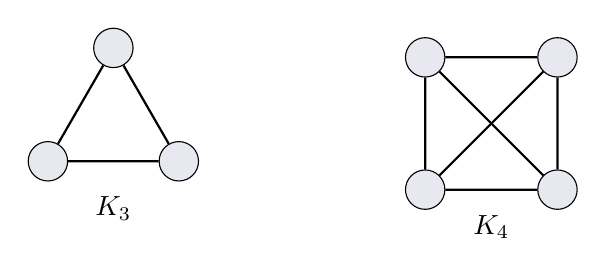
\begin{tikzpicture}[scale=1.2, node/.style={circle, draw, fill=MidnightBlue!10, inner sep=0pt, minimum size=5mm}]
  % K_3
  \begin{scope}[shift={(0,0)}]
    \node[node] (a) at (90:0.8) {};
    \node[node] (b) at (210:0.8) {};
    \node[node] (c) at (330:0.8) {};
    \draw[thick] (a) -- (b) -- (c) -- (a);
    \node at (0, -0.9) {$K_3$};
  \end{scope}

  % K_4
  \begin{scope}[shift={(4,0)}]
    \node[node] (1) at (-0.7,0.7) {};
    \node[node] (2) at (0.7,0.7) {};
    \node[node] (3) at (0.7,-0.7) {};
    \node[node] (4) at (-0.7,-0.7) {};
    \draw[thick] (1) -- (2) -- (3) -- (4) -- (1);
    \draw[thick] (1) -- (3);
    \draw[thick] (2) -- (4);
    \node at (0, -1.1) {$K_4$};
  \end{scope}
\end{tikzpicture}
\end{center}
\end{examples}

\begin{remark}[Regularität von $K_n$]
Der vollständige schlichte Graph $K_n$ ist $(n-1)$-regulär, da von jedem Knoten genau eine Kante zu den verbleibenden $n-1$ Knoten verläuft.
\end{remark}
\end{math-stroke}

\subsection{Teilgraphen und Erzeugte Teilgraphen}

\begin{spoken-clean}[00:56:56 - 00:58:54]
Ich mache wieder die nächste Definition: Wir nehmen jetzt an, dass wir Graphen $G = (V, E)$ und $G' = (V', E')$ haben, sodass $V' \subseteq V$ und $E' \subseteq E$ ist. Dann ist $G'$ ein Teilgraph von $G$. Wir schreiben $G' \subseteq G$.

Das ist auch klar: Wir nehmen einfach eine Teilmenge von Knoten, und alle Kanten in unserem Graphen $G'$ müssen auch Kanten in $G$ sein.

Gleichzeitig können wir auch, wenn wir einfach eine Menge von Knoten haben... Sei $U \subseteq V$. Der von $U$ erzeugte Teilgraph $G_U$ (oder $G|_U$) in $G$ ist der Graph mit Knoten $U$ und den Kanten $\{x, y\} \in E$, sodass $x, y \in U$ sind. Das heißt, wir nehmen alle Kanten dazu, die Knoten in $U$ verbinden.
\end{spoken-clean}

\begin{spoken-clean}[00:58:54 - 01:01:13]
Und gleichzeitig, wenn $F \subseteq E$ eine Teilmenge von Kanten ist: Der von $F$ erzeugte Teilgraph $G_F$ in $G$ ist der Teilgraph mit den Kanten $F$ und als Knoten einfach alle Knoten, die in diesen Kanten vorkommen. Das ist die Vereinigung von allen $\{x, y\}$, sodass $\{x, y\} \in F$ ist.

Gut, das ist ein Teilgraph.
\end{spoken-clean}

\begin{math-stroke}
\begin{definition}[Teilgraph]\label[definition]{def:teilgraph-formal}
Seien $G = (V, E)$ und $G' = (V', E')$ Graphen. $G'$ heißt \newterm{Teilgraph} von $G$ (geschrieben $G' \subseteq G$), falls gilt:
\[
V' \subseteq V \quad \text{und} \quad E' \subseteq E.
\]
\end{definition}

\begin{definition}[Knoteninduzierter Teilgraph]\label[definition]{def:knoteninduzierter-teilgraph}
Sei $G = (V, E)$ ein Graph und $U \subseteq V$. Der von $U$ \newterm{erzeugte (induzierte) Teilgraph} $G|_U \subseteq G$ (oder $G_U \subseteq G$) ist der Graph mit Knotenmenge $U$ und Kantenmenge:
\[
\bigl\{ \{x, y\} \in E \big| x, y \in U \bigr\}.
\]
\end{definition}

\begin{definition}[Kanteninduzierter Teilgraph]\label[definition]{def:kanteninduzierter-teilgraph}
Sei $G = (V, E)$ ein Graph und $F \subseteq E$. Der von $F$ \newterm{erzeugte Teilgraph} $G_F \subseteq G$ ist der Teilgraph von $G$ mit Kantenmenge $F$ und Knotenmenge:
\[
\bigcup_{\{x,y\}\in F}\{x,y\}.
\]
\end{definition}
\end{math-stroke}

\section{Wege, Pfade und Züge in Graphen}

\subsection{Pfeilzüge, Bahnen und Wirbel (Gerichtete Graphen)}

\begin{spoken-clean}[01:01:13 - 01:03:04]
Gut. Jetzt machen wir noch mehr Definitionen! Dazu würde ich wieder den Beamer verwenden.

Da geht es jetzt um Pfeilzüge. Wir machen das zuerst für Digraphen, weil Pfeile eine Richtung haben.

Wir sagen: Wenn wir einen Digraphen $G = (V, E)$ haben und $H \subseteq E$ eine nicht-leere, endliche Kantenteilmenge ist, sodass für ein $\ell \ge 1$ gilt: $|H| = \ell$ und $H = \{ (x_0, x_1), (x_1, x_2), \dots, (x_{\ell-1}, x_\ell) \}$, also immer der Endpunkt einer Kante der Anfangspunkt der nächsten ist, dann heißt der durch $H$ erzeugte Teilgraph $G_H$ Pfeilzug von $x_0$ nach $x_\ell$ der Länge $\ell$.

Ich mache da vielleicht noch ein Bild... \inlinemetanote{zeichnet eine Skizze an die Tafel}
\end{spoken-clean}

\begin{spoken-clean}[01:03:04 - 01:04:52]
Also ein Pfeilzug: Sagen wir, wir beginnen hier bei $x_0$, dann $x_1$, $x_2$, bis wir irgendwann bei $x_\ell$ ankommen... und dieser Teilgraph ist dann der Pfeilzug.

Hier bemerken wir: In dieser Definition müssen diese Kanten alle verschieden sein, weil die Kanten genau die Menge $H$ bilden. Es müssen also $\ell$ verschiedene Kanten sein.

Was aber nicht gefordert wird, ist, dass die Knoten verschieden sind. Man darf also mehrmals durch denselben Knoten gehen. Erlaubt ist zum Beispiel so etwas: \inlinemetanote{skizziert einen Knoten mit mehrfachem Durchgang} Das ist okay. Einfach die Kanten müssen alle verschieden sein. Das ist ein Pfeilzug.

Es gibt zwei verschiedene Arten von Pfeilzügen: Die einen sind offene Pfeilzüge, das heißt, falls $x_0 \neq x_\ell$, und geschlossene, falls $x_0 = x_\ell$.

Falls die $x_i$ paarweise verschieden sind, so heißt $G_H$ Bahn der Länge $\ell$ zwischen $x_0$ und $x_\ell$. Falls $x_0 = x_\ell$, die $x_i$ ansonsten aber paarweise verschieden sind, so heißt $G_H$ Wirbel.
\end{spoken-clean}

\begin{math-stroke}
\begin{definition}[Pfeilzug, Bahn und Wirbel]\label[definition]{def:pfeilzug}
Sei $G = (V, E)$ ein Digraph und sei $H \subseteq E$ eine nicht-leere, endliche Kantenteilmenge, sodass für ein $\ell \ge 1$ gilt: $|H| = \ell$ und $H = \{ (x_0, x_1), (x_1, x_2), \dots, (x_{\ell-1}, x_\ell) \}$. Der durch $H$ erzeugte Teilgraph $G_H$ heißt \newterm{Pfeilzug} von $x_0$ nach $x_\ell$ der Länge $\ell$.

Der Pfeilzug $G_H$ heißt:
\begin{itemize}
    \item \textbf{offener Pfeilzug}, falls $x_0 \neq x_\ell$,
    \item \textbf{geschlossener Pfeilzug}, falls $x_0 = x_\ell$.
\end{itemize}

Falls die $x_i$ paarweise verschieden sind, so heißt $G_H$ \newterm{Bahn} der Länge $\ell$ zwischen $x_0$ und $x_\ell$.
Falls $x_0 = x_\ell$, die $x_i$ ansonsten aber paarweise verschieden sind, so heißt $G_H$ \newterm{Wirbel}.
\end{definition}

\begin{center}
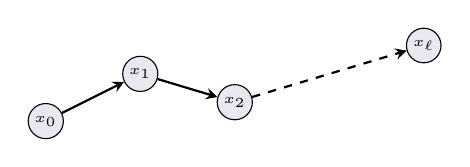
\begin{tikzpicture}[scale=1.2, ->, >=stealth, node/.style={circle, draw, fill=MidnightBlue!10, inner sep=1.5pt}]
  \node[node] (x0) at (0,0) {\tiny $x_0$};
  \node[node] (x1) at (1,0.5) {\tiny $x_1$};
  \node[node] (x2) at (2,0.2) {\tiny $x_2$};
  \node[node] (xl) at (4,0.8) {\tiny $x_\ell$};

  \draw[thick] (x0) -- (x1);
  \draw[thick] (x1) -- (x2);
  \draw[thick, dashed] (x2) -- (xl);
\end{tikzpicture}
\end{center}
\end{math-stroke}

\subsection{Kantenzüge, Wege und Kreise (Ungerichtete Graphen)}

\begin{spoken-clean}[01:04:52 - 01:06:39]
Gut, das sind Pfeilzüge. Dann gibt es Kantenzüge, und das ist eigentlich genau dieselbe Definition, diesmal einfach für... oh je, oh je... \inlinemetanote{bemerkt Tippfehler auf der Folie} Okay, das muss man fast korrigieren jetzt... \inlinemetanote{korrigiert die Projektionsfolie am Laptop}

Wenn wir mit ungerichteten Graphen arbeiten, dann heißt das Ganze Kantenzüge anstatt Pfeilzüge. Gut, jetzt haben wir das auch. Das war so falsch, solche Tippfehler darf man nicht stehen lassen.

Also, wenn wir einen ungerichteten Graphen haben und eine nicht-leere, endliche Kantenteilmenge $H$ mit $|H| = \ell$ für ein $\ell \ge 1$ und $H = \{\{x_0, x_1\}, \dots, \{x_{\ell-1}, x_\ell\}\}$: Dann heißt der durch $H$ erzeugte Teilgraph $G_H$ Kantenzug von $x_0$ nach $x_\ell$ der Länge $\ell$.

Und auch hier wieder: Ein Kantenzug heißt offen oder geschlossen.

Und anstelle von Bahn und Wirbel sagen wir Weg oder Kreis. Das sind einfach zwei verschiedene Welten, aber es ist für ungerichtete Graphen genau dieselbe Definition, einfach eine andere Notation.
\end{spoken-clean}

\begin{math-stroke}
\begin{definition}[Kantenzug, Weg und Kreis]\label[definition]{def:kantenzug}
Sei $G = (V, E)$ ein ungerichteter Graph und sei $H \subseteq E$ eine nicht-leere, endliche Kantenteilmenge, sodass für ein $\ell \ge 1$ gilt: $|H| = \ell$ und $H = \{ \{x_0, x_1\}, \{x_1, x_2\}, \dots, \{x_{\ell-1}, x_\ell\} \}$. Der durch $H$ erzeugte Teilgraph $G_H$ heißt \newterm{Kantenzug} von $x_0$ nach $x_\ell$ der Länge $\ell$.

Der Kantenzug $G_H$ heißt:
\begin{itemize}
    \item \textbf{offener Kantenzug}, falls $x_0 \neq x_\ell$,
    \item \textbf{geschlossener Kantenzug}, falls $x_0 = x_\ell$.
\end{itemize}

Falls die $x_i$ paarweise verschieden sind, so heißt $G_H$ \newterm{Weg} der Länge $\ell$ zwischen $x_0$ und $x_\ell$.
Falls $x_0 = x_\ell$, die $x_i$ ansonsten aber paarweise verschieden sind, so heißt $G_H$ \newterm{Kreis}.
\end{definition}
\end{math-stroke}

\begin{spoken-clean}[01:06:39 - 01:07:32]
Da können wir das noch kurz aufschreiben. Wir haben hier gerichtet und ungerichtet:
\inlinemetanote{schreibt die Gegenüberstellungstabelle an die Tafel}
\end{spoken-clean}

\begin{math-stroke}[Übersichtstabelle: Gerichtete vs. Ungerichtete Begriffe]
\begin{center}
\begin{tabular}{l | l}
    \toprule
    \textbf{Gerichtet (Digraph)} & \textbf{Ungerichtet} \\
    \midrule
    Pfeilzug & Kantenzug \\
    Bahn     & Weg \\
    Wirbel   & Kreis \\
    \bottomrule
\end{tabular}
\end{center}
\end{math-stroke}

\subsection{Pfeilfolgen}

\begin{spoken-clean}[01:07:32 - 01:08:48]
Gut, und das nächste Konzept sind noch Pfeilfolgen.

Das ist wieder eine zusätzliche Definition: Wenn wir einen Digraphen haben, also wieder einen gerichteten Graphen, dann sagen wir: Eine Folge der Länge $\ell$ von Kanten $(x_0, x_1), (x_1, x_2), \dots, (x_{\ell-1}, x_\ell)$, in der Kanten auch mehrfach vorkommen können, heißt eine Pfeilfolge von $x_0$ nach $x_\ell$ der Länge $\ell$.

Genau, eine Pfeilfolge ist also sehr ähnlich wie ein Pfeilzug, nur dürfen hier die Kanten auch mehrfach vorkommen.
\end{spoken-clean}

\begin{math-stroke}
\begin{definition}[Pfeilfolge]\label[definition]{def:pfeilfolge}
Sei $G = (V, E_0, \dots, E_k)$ ein Digraph. Eine Folge der Länge $\ell$ von Kanten $(x_0, x_1), (x_1, x_2), \dots, (x_{\ell-1}, x_\ell)$, in der Kanten auch mehrfach vorkommen können, heißt eine \newterm{Pfeilfolge} von $x_0$ nach $x_\ell$ der Länge $\ell$.
\end{definition}
\end{math-stroke}

\section{Anzahl der Pfeilfolgen und die Adjazenzmatrix}

\subsection{Pfadzählung mittels Matrixpotenzen (Proposition~\ref{prop:adjazenzmatrix-potenz-pfeilfolgen})}

\begin{spoken-clean}[01:08:48 - 01:11:54]
Und jetzt endlich einmal noch ein nettes Resultat! Dass wir endlich einmal noch ein Resultat haben und nicht nur Definitionen.

Das ist Proposition~\ref{prop:adjazenzmatrix-potenz-pfeilfolgen}. Die sagt aus: Sei $V = \{v_1, \dots, v_n\}$ und $G = (V, E_0, \dots, E_k)$ ein Digraph mit Adjazenzmatrix $A = A(G)$.

Schreibe $A^k = (a_{ij}^{(k)})$. Dann ist $a_{ij}^{(k)}$ die Anzahl der verschiedenen Pfeilfolgen von $v_i$ nach $v_j$ der Länge $k$.

Okay, das heißt: Indem wir diese Matrix mit sich selbst multiplizieren, erhalten wir eine nette kombinatorische Interpretation dafür, was diese Einträge der Matrix bedeuten.
\end{spoken-clean}

\begin{math-stroke}
\begin{proposition}\label[proposition]{prop:adjazenzmatrix-potenz-pfeilfolgen}
Sei $V = \{v_1, \dots, v_n\}$ und $G = (V, E_0, \dots, E_m)$ ein Digraph mit Adjazenzmatrix $A = A(G)$ \inlinemetanote{[Anmerkung: Auf der Folie heisst der Index der Kantenrelationen ebenfalls $k$; da $k$ hier zugleich der Exponent von $A^k$ ist, wird er zur Vermeidung der Doppelbelegung zu $m$ umbenannt.]}. Schreibe $A^k = (a_{ij}^{(k)})$.

Dann ist $a_{ij}^{(k)}$ die Anzahl der verschiedenen Pfeilfolgen von $v_i$ nach $v_j$ der Länge $k$.
\end{proposition}
\end{math-stroke}

\begin{spoken-clean}[01:11:54 - 01:14:32]
Vielleicht schauen wir uns kurz noch ein paar ganz einfache Beispiele an.

Wenn wir hier zum Beispiel zwei Knoten haben und zwei Kanten von $1$ nach $2$ gehen sowie eine Kante von $2$ nach $1$:

Was ist die Adjazenzmatrix? Das ist $A = \begin{pmatrix} 0 & 2 \\ 1 & 0 \end{pmatrix}$. Es gibt keine Kante von $1$ zu sich selbst, es gibt $2$ von $1$ nach $2$, es gibt $1$ von $2$ nach $1$ und keine von $2$ zu sich selbst.

Wir sehen hier: Für $k=1$ gilt das natürlich schon per Definition: Es gibt $2$ Möglichkeiten, von $1$ nach $2$ zu laufen, und $1$ Möglichkeit, von $2$ nach $1$ zu laufen.

Wenn wir jetzt $A^2$ ausrechnen, dann erhalten wir $\begin{pmatrix} 2 & 0 \\ 0 & 2 \end{pmatrix}$. Und da sehen wir: Um von $1$ zu sich selbst zu laufen, gibt es $2$ Möglichkeiten, nämlich $1 \to 2 \to 1$. Und um von $2$ zu sich selbst zu laufen, gibt es auch $2$ Möglichkeiten. Aber es gibt keine Möglichkeit, von $1$ nach $2$ mit einer Pfeilfolge der Länge $2$ zu laufen.

Und ähnlich ist $A^3 = \begin{pmatrix} 0 & 4 \\ 2 & 0 \end{pmatrix}$. Da sehen wir wieder: Okay, wenn man eine Pfeilfolge der Länge $3$ nimmt, kommt man wieder nur von $1$ nach $2$ und von $2$ nach $1$. Und es gibt genau $4$ Möglichkeiten, von $1$ nach $2$ zu gehen. Hingegen gibt es um von $2$ nach $1$ mit Länge $3$ zu laufen nur $2$ Möglichkeiten.
\end{spoken-clean}

\begin{math-stroke}
\begin{example}[Matrixpotenzen für 2-Knoten-Digraphen]
\label[example]{ex:matrixpotenzen-2knoten}
Sei $V = \{1, 2\}$ und $E$ bestehe aus zwei Kanten von $1$ nach $2$ sowie einer Kante von $2$ nach $1$:

\begin{center}
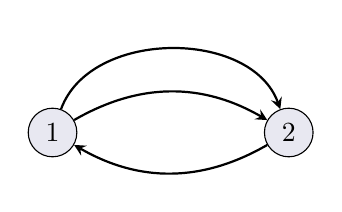
\begin{tikzpicture}[scale=1.2, ->, >=stealth, node/.style={circle, draw, fill=MidnightBlue!10, font=\bfseries}]
  \node[node] (1) at (0,0) {$1$};
  \node[node] (2) at (2.5,0) {$2$};

  \draw[thick] (1) to[bend left=30] (2);
  \draw[thick] (1) to[bend left=70] (2);
  \draw[thick] (2) to[bend left=30] (1);
\end{tikzpicture}
\end{center}

Die Adjazenzmatrix und ihre ersten Potenzen lauten:
\begin{align*}
A &= \begin{pmatrix} 0 & 2 \\ 1 & 0 \end{pmatrix}, \\[6pt]
A^2 &= \begin{pmatrix} 0 & 2 \\ 1 & 0 \end{pmatrix} \begin{pmatrix} 0 & 2 \\ 1 & 0 \end{pmatrix} = \begin{pmatrix} 2 & 0 \\ 0 & 2 \end{pmatrix}, \\[6pt]
A^3 &= A^2 \cdot A = \begin{pmatrix} 2 & 0 \\ 0 & 2 \end{pmatrix} \begin{pmatrix} 0 & 2 \\ 1 & 0 \end{pmatrix} = \begin{pmatrix} 0 & 4 \\ 2 & 0 \end{pmatrix}.
\end{align*}
\end{example}
\end{math-stroke}

\subsection{Induktionsbeweis von Proposition~\ref{prop:adjazenzmatrix-potenz-pfeilfolgen}}

\begin{proof}[Beweis von Proposition \ref{prop:adjazenzmatrix-potenz-pfeilfolgen}]
\begin{spoken-clean}[01:14:32 - 01:17:39]
Der Beweis folgt per Induktion nach $k$.

Für $k = 1$ ist das genau gemäß der Definition der Adjazenzmatrix $A(G)$.

Induktionsschritt: Wir nehmen an, die Aussage stimmt für $k$, und wir müssen sie für $k+1$ beweisen.

Per Induktionsannahme wissen wir: Für $1 \le i, \ell \le n$ ist $a_{i\ell}^{(k)}$ die Anzahl der Pfeilfolgen der Länge $k$ von $v_i$ nach $v_\ell$.

Für $1 \le i, j, \ell \le n$ ist $a_{i\ell}^{(k)} \cdot a_{\ell j}^{(1)}$ die Anzahl der Pfeilfolgen der Länge $k+1$ von $v_i$ nach $v_j$ via $v_\ell$ im letzten Schritt.
\end{spoken-clean}

\begin{spoken-clean}[01:17:39 - 01:19:44]
Okay, wenn wir also nur die Pfeilfolgen anschauen, die von $v_i$ nach $v_j$ gehen und im letzten Schritt über $v_\ell$ gehen sollen, dann ist das genau das Produkt. Hier können wir eine der $a_{i\ell}^{(k)}$ Pfeilfolgen auswählen, und dann haben wir hier nochmals $a_{\ell j}^{(1)}$ Möglichkeiten.

Und somit erhalten wir, dass die Anzahl der Pfeilfolgen von $v_i$ nach $v_j$ der Länge $k+1$ genau die Summe von $\ell=1$ bis $n$ über $a_{i\ell}^{(k)} \cdot a_{\ell j}^{(1)}$ ist:
\[
a_{ij}^{(k+1)} = \sum_{\ell=1}^n a_{i\ell}^{(k)} a_{\ell j}^{(1)}.
\]
Das ist per Definition genau die Matrixmultiplikation $A^{k+1} = A^k \cdot A$. Das beweist die Proposition.
\end{spoken-clean}

\begin{math-stroke}[Induktionsbeweis von Proposition~\ref{prop:adjazenzmatrix-potenz-pfeilfolgen}]
\textbf{Induktionsanfang ($k=1$):} Für $k=1$ gilt $A^1 = A$. Nach Definition der Adjazenzmatrix ist $a_{ij}^{(1)}$ die Anzahl der Kanten (Pfeilfolgen der Länge 1) von $v_i$ nach $v_j$.

\textbf{Induktionsschritt ($k \to k+1$):} 
Wir nehmen an, die Behauptung gilt für $k \ge 1$.
Seien $v_i, v_j \in V$. Jede Pfeilfolge der Länge $k+1$ von $v_i$ nach $v_j$ besteht aus einer Pfeilfolge der Länge $k$ von $v_i$ zu einem Zwischenknoten $v_\ell$ und einer anschließenden Kante von $v_\ell$ nach $v_j$.

Nach Induktionsvoraussetzung gibt es genau $a_{i\ell}^{(k)}$ Pfeilfolgen der Länge $k$ von $v_i$ nach $v_\ell$, und nach Definition gibt es $a_{\ell j}^{(1)}$ Kanten von $v_\ell$ nach $v_j$.
Nach der Pfadregel gibt es über den festen Knoten $v_\ell$ somit genau:
\[
a_{i\ell}^{(k)} \cdot a_{\ell j}^{(1)}
\]
Pfeilfolgen der Länge $k+1$.
Summiert man über alle möglichen Zwischenknoten $v_\ell \in \{v_1, \dots, v_n\}$, so ergibt sich die Gesamtzahl aller Pfeilfolgen der Länge $k+1$ von $v_i$ nach $v_j$:
\[
\sum_{\ell=1}^n a_{i\ell}^{(k)} a_{\ell j}^{(1)} = (A^k \cdot A)_{ij} = a_{ij}^{(k+1)}.
\]
Dies schließt den Induktionsbeweis ab.
\end{math-stroke}
\end{proof}

\begin{spoken-clean}[01:19:44 - 01:25:38]
Im Skript haben wir noch ein komplizierteres Beispiel, das ganz nett ist: den Graphen, den wir vorher gesehen haben.

Wenn man da die Adjazenzmatrix hoch $4$ rechnet, dann erhält man diese Matrix. Und aus dieser Matrix kann man jetzt tatsächlich ablesen, wie viele mögliche Pfeilfolgen es zwischen je zwei von diesen Knoten gibt.

Zum Beispiel vom Knoten $6$ zum Knoten $5$: Das ist hier diese Zahl da unten, und da wissen wir jetzt, es gibt $4$.

Gut. Wir waren heute etwas langsamer als gedacht, aber das ist nicht schlimm; wir machen nächste Woche noch mit den Graphen fertig. Vielen Dank und ein schönes Wochenende! \inlinemetanote{Vorlesung endet; Studenten klatschen}
\end{spoken-clean}

\begin{math-stroke}[Komplexes Beispiel für $A^4$]
\begin{meta-note}[Projizierte Folie: $A^4$ für einen 6-Knoten-Digraphen]
Für den vorhin projizierten Digraphen mit $6$ Knoten ergibt die Berechnung der vierten Potenz der Adjazenzmatrix:
\[
A^4 = \begin{pmatrix}
5 & 7 & 4 & 7 & 5 & 1 \\
3 & 6 & 3 & 7 & 4 & 2 \\
4 & 9 & 3 & 14 & 7 & 7 \\
1 & 3 & 2 & 3 & 1 & 1 \\
1 & 4 & 1 & 11 & 4 & 6 \\
3 & 4 & 1 & 5 & 4 & 2
\end{pmatrix}.
\]
Der Eintrag $a_{6,5}^{(4)} = 4$ bestätigt, dass es genau $4$ verschiedene Pfeilfolgen der Länge $4$ vom Knoten $6$ zum Knoten $5$ gibt.
\end{meta-note}
\end{math-stroke}

\begin{ai-note}[{$A^4$ vermutlich inkonsistent mit dem Graphen weiter oben --- Sonnet 5.x / Medium}]
Aus der Kantenmenge des früher gezeichneten 6-Knoten-Digraphen (TikZ-Bild, Abschnitt "Komplexeres Beispiel eines gerichteten Multigraphen") hat Knoten $3$ außer seiner eigenen Schlinge keine eingehenden Kanten, weshalb $a_{i,3}^{(k)}=0$ für alle $i\neq 3$ und alle $k$ gelten müsste --- auch für $A^4$. Die hier angegebene Matrix widerspricht dem (u.\,a.\ Spalte 3 sowie der hervorgehobene Wert $a_{6,5}^{(4)}=4$, der bei diesem Graphen $0$ sein sollte). Zu prüfen anhand der Originalfolie/des Videos (ca. 01:19:44--01:25:38), ob dem TikZ-Bild Kanten fehlen oder die $A^4$-Werte fehlerhaft übernommen wurden.
\end{ai-note}

\begin{nice-box}[Zusammenfassung der Kernkonzepte]
\begin{itemize}
    \item \textbf{Graph \& Kantenrelationen:} Ein Graph $G = (V, E)$ besteht aus einer Knotenmenge $V$ und Kanten $E \subseteq V \times V$. Man unterscheidet gerichtete Graphen (Digraphen), ungerichtete Graphen ($E$ symmetrisch), Schlingen ($(x,x) \in E$), Mehrfachkanten (Multigraphen) und schlichte Graphen (schlingen- und mehrfachkantenfrei).
    \item \textbf{Adjazenzmatrix $A(G)$:} Für $V = \{v_1, \dots, v_n\}$ gibt $a_{ij}$ die Anzahl der Kanten von $v_i$ nach $v_j$ an. $A(G)$ ist symmetrisch genau dann, wenn $G$ ungerichtet ist, und $G$ ist schlingenfrei genau dann, wenn $\operatorname{Spur}(A(G)) = 0$.
    \item \textbf{Knotengrad \& Halbgrade:} In Digraphen unterscheiden wir den Ausgangsgrad $\operatorname{deg}^+(x)$ und Eingangsgrad $\operatorname{deg}^-(x)$. Im ungerichteten Fall zählt $\operatorname{deg}(x)$ die inzidenten Kantenenden, wobei Schlingen doppelt zählen.
    \item \textbf{Spezielle Graphenklassen:} Ein $r$-regulärer Graph besitzt an jedem Knoten den Grad $r$. Der vollständige schlichte Graph $K_n$ besitzt alle Kanten ohne Schlingen und ist $(n-1)$-regulär.
    \item \textbf{Züge, Wege \& Pfade:} Pfeilzüge (Digraphen) und Kantenzüge (ungerichtet) bestehen aus paarweise verschiedenen Kanten. Sind zusätzlich die Knoten paarweise verschieden, spricht man von Bahnen bzw. Wegen (offen) oder Wirbeln bzw. Kreisen (geschlossen).
    \item \textbf{Matrixpotenzen \& Pfadanzahl (Proposition~\ref{prop:adjazenzmatrix-potenz-pfeilfolgen}):} Der Eintrag $a_{ij}^{(k)}$ der $k$-ten Matrixpotenz $A^k$ entspricht exakt der Anzahl aller Pfeilfolgen der Länge $k$ vom Knoten $v_i$ zum Knoten $v_j$.
\end{itemize}
\end{nice-box}